


\section{Introduction}
\label{sec:intro}

% \red{PLEASE add missing references in this section}

Deep neural networks have demonstrated remarkable performance when the training and test domains follow the same data distribution \cite{lu2022survey}. However, their accuracy drops significantly when testing data suffers from distribution shifts \cite{lu2022survey,liang2024comprehensive}.
% , which is frequently encountered in the real world~\cite{hendrycks2019benchmarking}. 
To address this, numerous attempts have been explored, such as unsupervised domain adaptation \cite{ge2023unsupervised}, source-free domain adaptation~\cite{li2024comprehensive}, and domain generalization \cite{zhou2022domain}. However, in dynamic applications like autonomous driving, environmental conditions are constantly evolving, causing continuous data distribution shifts~\cite{li2023lwsis,sakaridis2021acdc}. To maintain stable and excellent performance, models need to adapt continuously to new conditions—an especially challenging task given the unpredictability of new environments~\cite{pan2020unsupervised}.  

% However, these methods fail to perform well when the domain shift changes constantly in an unpredictable manner. 

% \red{pls use another example, simulation and real-world is too ideal} 


% \For example, each domain developed a lung diagnosis model tailored to a specific hospital using its own CT images. Although the collected images represent the same disease, the data distributions vary across domains due to differences in the CT equipment used by different hospitals. Consequently, a model may struggle to perform effectively on data from another domain because of these domain shifts. 
% Deep neural networks (DNNs) perform perfectly when the training and test domains share the same data distribution. However, the performance drops dramatically when domain shifts exist~\cite{lu2022survey,liang2024comprehensive}. A typical example of domain shifts is the gap between a simulation environment and a real scenario for the same robot~\cite{kim2022ev}. In real-world applications like autonomous driving, the perceived scenarios change continuously, leading to persistent variations in data distribution~\cite{li2023lwsis,sakaridis2021acdc}. Therefore, a computational model must constantly adapt to new conditions. This requirement is too difficult to satisfy since the new environment is unpredictable~\cite{pan2020unsupervised}. Recently, test-time adaptation (TTA) has emerged as a promising paradigm for addressing such challenges in an online manner~\cite{wang2020tent,niu2023towards,lee2024entropy,liang2024comprehensive}.


\begin{figure*}[t]
\centering
% 子图1
\begin{subfigure}[t]{0.33\textwidth} 
    \centering
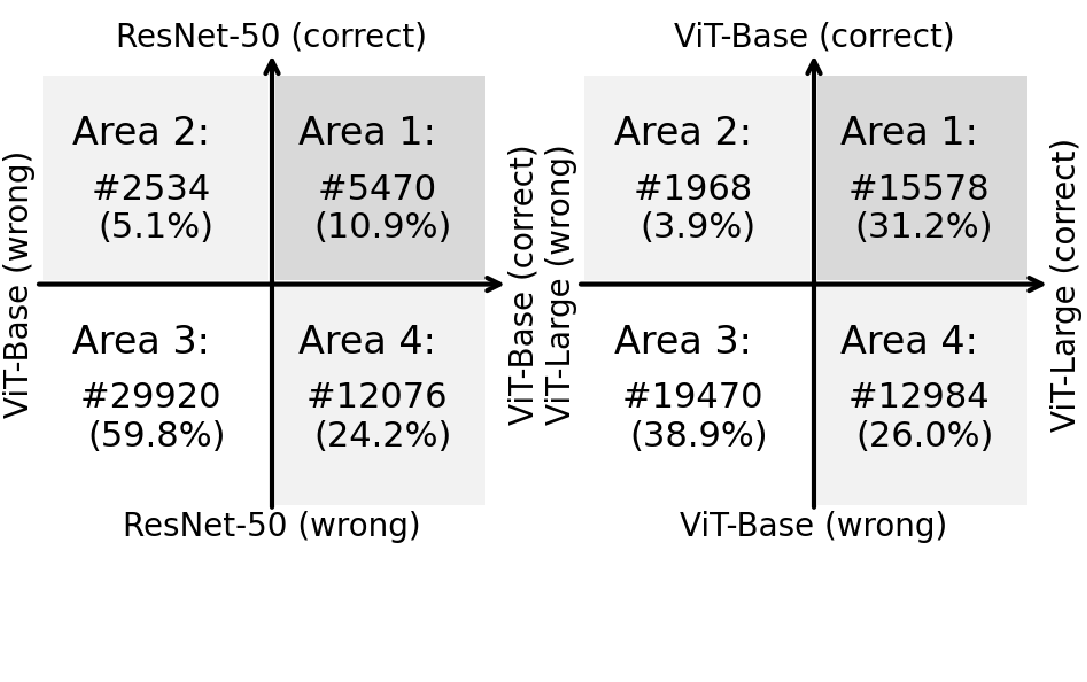
\includegraphics[width=\linewidth]{sec/fig1a_2.pdf}
\subcaption{Distinctness of model predictions
}
    \label{fig1a}
\end{subfigure}
\hfill
% 子图2
\begin{subfigure}[t]{0.34\textwidth}
    \centering
    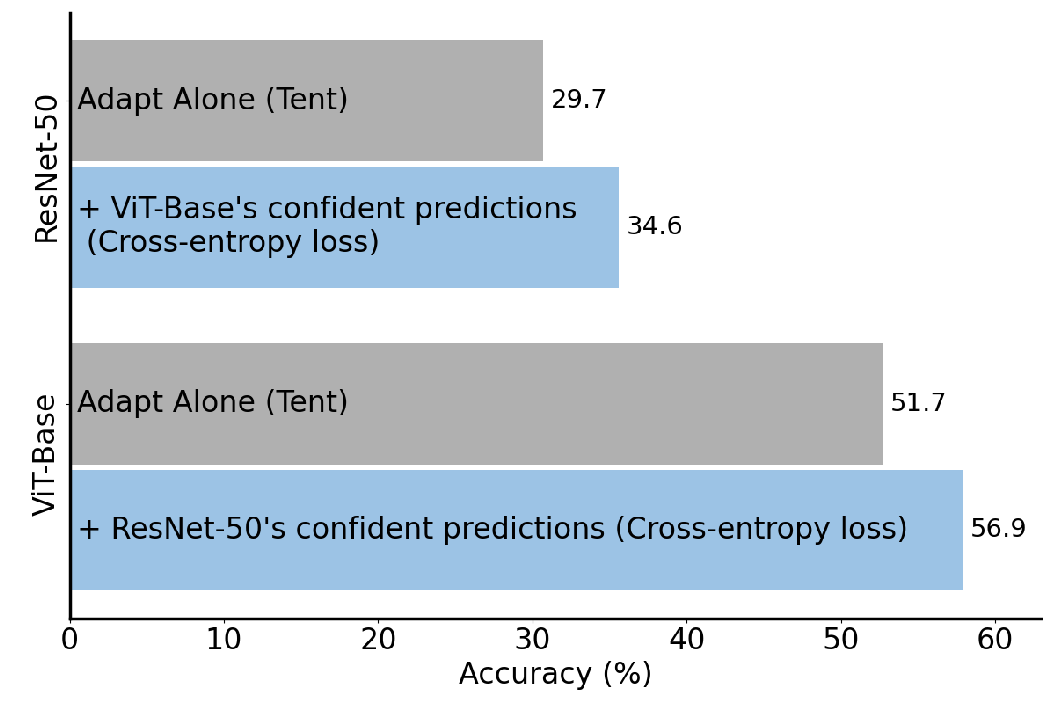
\includegraphics[width=\linewidth]{sec/fig1b_2.pdf}
    \subcaption{Benefits of complementary knowledge
}
    \label{fig1b}
\end{subfigure}
\hfill
% 子图3
\begin{subfigure}[t]{0.32\textwidth}
    \centering
    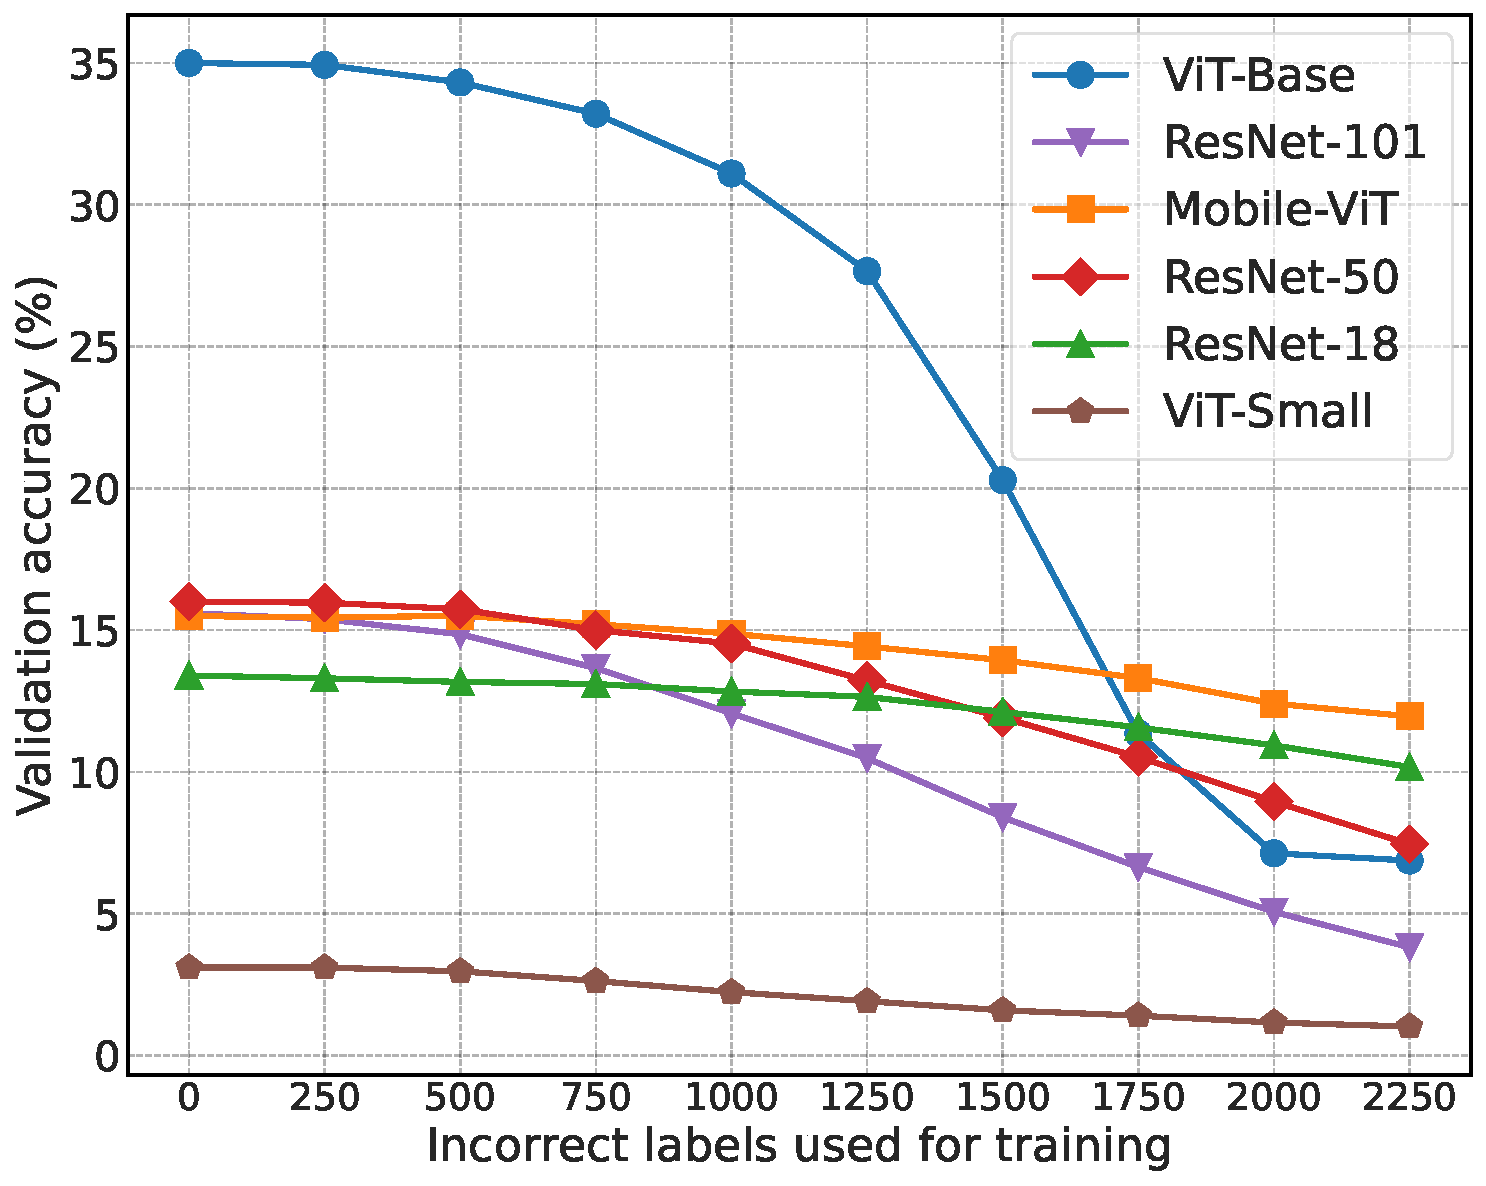
\includegraphics[width=\linewidth]{sec/fig1c_2.pdf}
    \subcaption{TTA robustness against noisy labels 
}
    \label{fig1c}
\end{subfigure}

\vspace{-0.1in}
\caption{Motivation for COCA. (a) Pre-trained models exhibit distinct strengths due to differences in training strategies, architectures, or sizes. (b) TTA~\cite{wang2020tent}, using complementary confident predictions from another model, significantly enhances adaptation performance. (c) Larger models are more vulnerable to erroneous guidance than smaller ones, highlighting differences in robustness during test time. Results are based on predicting ImageNet-C (Gaussian noise, level 5) with various ResNet-based~\cite{he2016deep} and Transformer-based~\cite{dosovitskiy2020image} models. Confident samples are filtered using an entropy threshold of 0.4*ln1000 following EATA~\cite{niu2022efficient}.}
\label{motifig1}
\vspace{-0.2in}
\end{figure*}


% \begin{figure*}[t]
%     \centering  
%     \includegraphics[width=\linewidth]{sec/fig1_3.7.pdf}
%     \vspace{-0.3in}
%     \caption{Motivation for COCA. (a) Pre-trained models exhibit distinct strengths due to differences in training strategies, architectures, and sizes. (b) TTA~\cite{wang2020tent}, using complementary confident predictions from another model, significantly enhances adaptation performance. (c) Larger models are more vulnerable to erroneous guidance than smaller ones, highlighting differences in robustness during test time. Results are based on predicting ImageNet-C (Gaussian noise, level 5) with various ResNet-based and Transformer-based models. Confident samples are filtered using a threshold of 0.4*ln1000 as defined by EATA~\cite{niu2022efficient}.}
%     \vspace{-0.15in}
%     \label{motifig1}
% \end{figure*}

% (a) Despite substantial differences in model architecture, parameter size, and TTA performance, pre-trained models always exhibit complementary knowledge and unique strengths. (b) Larger models are more susceptible to erroneous supervision, highlighting their varying robustness during test-time adaptation. (c) Motivated by these observations we introduce a simple co-learning strategy for TTA~\cite{wang2020tent}, where confident predictions from another model, filtered with a threshold of 0.4*ln1000 (as defined by EATA~\cite{niu2022efficient}), are used as pseudo-labels. This approach leads to a significant improvement in adaptation performance.




% \begin{figure}[t]
%     \centering  
%     \includegraphics[width=\linewidth]{sec/fig1.pdf}
%     \caption{Motivation of Test-Time Co-Learning. (a) Each model possesses its own confident predictions (knowledge), which are both shared with and complementary to the other. \# The number of samples is counted based on the source model. (b) TTA~\cite{wang2020tent} using complementary confident predictions from the other model is able to enhance adaptation performance a lot. Results obtained on ImageNet-C (Gaussian noise, level 5) with ViT-B (ViT-Base) and RN-50 (ResNet-50). }
%     \vspace{-0.1in}
%     \label{motifig1}
% \end{figure}
% An illustration showing the motivation of this work. (a) shows that two models produce different confident level predictions (confident and unconfident is divided by threshold 0.4*ln(1000) follow EATA~\cite{niu2022efficient} setting)for the same 50000 samples (Gauss noise of ImageNet-C). (b) demonstrates that one model can achieve significant improvement by learning from another(+ ViT-B/RN-50's knowledge denotes using its predictions as pseudo-labels for an extra cross-entropy loss).

% \red{unsupervised domain adaptation (UDA) aims to transfer models from a source domain to a target domain without access to labeled target data. This is typically achieved by learning domain-invariant feature representations \cite{li2020model, liang2020we} or through adversarial alignment \cite{liu2021adversarial}. Building upon this foundation, the fully test-time adaptation (TTA) setting was proposed \cite{wang2020tent}, where no source data or supervision is available during testing. In this setting, the model must adapt to the target domain in real-time, without revisiting the same target samples. This setup reflects the need for adaptation in practical, real-world scenarios where the target data is continuously changing and no labeled data is available.}
% \red{PLEASE introduce other works for addressing domain shifts such as unsupervised domain adaptation, domain generalization, etc., then introducing TTA: how TTA works and its advantages over prior methods, our introduction is too short}

% To achieve this, Recently, Test-time adaptation (TTA) has gained considerable attention as a promising approach for handling these shifts and challenges in real time~\cite{wang2020tent,niu2023towards,lee2024entropy,liang2024comprehensive}.

Recently, test-time adaptation (TTA) has emerged as a promising paradigm for tackling these challenges~\cite{sun2020test,liu2021ttt++,niu2023towards,lee2024entropy,liang2024comprehensive}. By directly leveraging test data through self-supervised or unsupervised objectives, TTA benefits from an online, source-free approach. This is especially true for fully TTA methods~\cite{wang2020tent,niu2022efficient}, which can be applied to any pre-trained model, thereby significantly broadening its appeal in real-world applications compared to earlier techniques. 
However, existing TTA methods~\cite{wang2020tent,niu2022efficient,lee2024entropy} typically focus on single-model adaptation and are excessively sensitive to pseudo label noise. 
Motivated by the success of co-learning~\cite{zhang2018deep} and knowledge distillation~\cite{hinton2015distilling,mirzadeh2020improved} in conventional supervised learning, we pose a natural question: Can co-learning also enhance TTA? 

To investigate this, we conduct two key experiments to examine the complementary capabilities of different models during TTA, revealing that: 1) \textit{Complementary knowledge between models}: As from Fig.~\ref{motifig1}(a), we show that different models can yield complementary predictions for the same data due to variations in training strategies, architectures, or sizes.
By leveraging the complementary confident samples from the other model to construct a pseudo cross-entropy loss during TTA, we significantly improve the adaptation performance on both the large and small model compared to Tent~\cite{wang2020tent}. 2) \textit{Differential robustness of models in TTA}: We evaluate the TTA robustness of various models by adapting them to test samples with randomly erroneous labels, using the same learning rate as in Tent~\cite{wang2020tent}. While larger models initially yield higher accuracy, they are more sensitive to incorrect pseudo labels during TTA, as shown in Fig.\ref{motifig1}(c). These findings indicate the potential of a small model to significantly improve the TTA performance and robustness of a larger model through cross-model co-learning.


% Recently, test-time adaptation (TTA) has emerged as a promising paradigm for addressing such challenges~\cite{sun2020test,liu2021ttt++,niu2023towards,lee2024entropy,liang2024comprehensive}, which directly learns from test data through self-supervised or unsupervised objectives. Benefiting from its online and unsupervised nature without access to source data, particularly of fully TTA methods~\cite{wang2020tent,niu2022efficient} that can be applied to any pre-trained model, TTA has broadened its practical appeal in real-world applications compared to prior techniques. Though effective at handling the domain shift issue, existing TTA methods~\cite{wang2020tent,niu2022efficient,lee2024entropy} typically focus on single-model adaptation. Inspired by the success of co-learning~\cite{zhang2018deep} and knowledge distillation~\cite{hinton2015distilling,mirzadeh2020improved,beyer2022knowledge} in conventional supervised learning, we ask: can co-learning also be effective for TTA in an online unsupervised setting? 

% To explore this, we first compare how different models predict identical inputs to assess their complementary knowledge. Using ResNet~\cite{he2016deep} and Transformer~\cite{dosovitskiy2020image} backbones, Fig.~\ref{motifig1}(a) shows that different models yield distinct predictions for the same data without adaptation, reflecting differences in training strategies, architectures, or sizes. Building on this observation, we leverage these complementary samples to construct a pseudo cross-entropy loss that assists the other model during TTA, using Tent~\cite{wang2020tent}. As illustrated in Fig.~\ref{motifig1}(b), incorporating complementary information from another model significantly enhances the adaptation performance of the current model. Additionally, we guide each model’s test-time adaptation using randomly erroneous labels. In each training and validation round, there is no overlap between samples. Fig.\ref{motifig1}(c) shows that larger models are more sensitive to incorrect guidance than smaller ones, indicating varying robustness during test time. These findings highlight the potential of cross-model co-learning to enhance TTA.


% (a) Despite substantial differences in model architecture, parameter size, and TTA performance, pre-trained models always exhibit complementary knowledge and unique strengths. (b) Larger models are more susceptible to erroneous supervision, highlighting their varying robustness during test-time adaptation. (c) Motivated by these observations we introduce a simple co-learning strategy for TTA~\cite{wang2020tent}, where confident predictions from another model, filtered with a threshold of 0.4*ln1000 (as defined by EATA~\cite{niu2022efficient}), are used as pseudo-labels. This approach leads to a significant improvement in adaptation performance.


In light of the above motivation, we propose a novel approach called COCA — \textbf{c}ross-m\textbf{o}del \textbf{c}o-le\textbf{a}rning for enhanced TTA, which mainly consists of two strategies, \ie, co-adaptation and self-adaptation. Co-adaptation integrates complementary knowledge between models during TTA to reduce individual biases. To achieve this, we introduce an adaptive temperature-scaled marginal entropy loss to promote mutual learning. The adaptive temperature is automatically determined via an anchor-guided alignment loss, using the larger model as an anchor. This enables robust knowledge aggregation, particularly when there is a significant size disparity between models, or the learning signals from the smaller models can otherwise be overstated or overlooked. Additionally, we propose a cross-model knowledge distillation loss, leveraging combined predictions as pseudo-labels to supervise both models and maximize the effective use of cross-model knowledge. On the other hand, self-adaptation allows each model to independently adapt using existing unsupervised learning objectives from single-model TTA, enhancing each model’s unique strengths and fostering diverse adaptation to the target domain. 
% Finally, the predictions from both adapted models can be either independently or adaptively ensembled to generate the final prediction for the test data.


% 1) Co-adaptation, which integrates the complementary knowledge between models for TTA to mitigate individual model biases; and 2) Self-adaptation, which enhances each model’s unique strengths by unsupervised learning, enabling diverse adaptation to the target domain.
% Beyond co-adaptation, the self-adaptation strategy allows each model to independently adapt within its own branch using existing single-model TTA objectives. This approach enhances each model’s unique strengths through unsupervised learning, facilitating diverse adaptation to the target domain  



% Based on co-adaptation, COCA integrates the complementary knowledge between models to mitigate individual model biases. Based on self-adaptation, COCA enhances each model’s unique strengths by unsupervised learning, enabling diverse adaptation to the target domain. Then, the predictions from both adapted models are adaptively ensembled to produce final predictions for the test data.



% In light of the above motivation, we propose a novel approach called COCA — \textbf{c}ross-m\textbf{o}del \textbf{c}o-le\textbf{a}rning for enhanced TTA, which aims to explore the mutual improvement across different models to better fit the target data. The motivation of this paper is illustrated in Fig.~\ref{motifig1}, where ViT-B, RN-50, and CE represent ViT-Base, ResNet-50, and Cross-Entropy, respectively. COCA mainly consists of two strategies, i.e., co-adaptation and self-adaptation. Based on co-adaptation, COCA integrates the complementary knowledge between models to mitigate individual model biases. Based on self-adaptation, COCA enhances each model’s unique strengths by unsupervised learning, enabling diverse adaptation to the target domain. Then, the predictions from both adapted models are adaptively ensembled to produce final predictions for the test data.


% COCA employs two main strategies: 1) Co-adaptation, which integrates the complementary knowledge between models for TTA to mitigate individual model biases; and 2) Self-adaptation, which enhances each model’s unique strengths by unsupervised learning, enabling diverse adaptation to the target domain. Then, we adaptively ensemble the predictions from both adapted models to achieve more robust predictions for the test data.

% In light of the above motivation, we propose a novel approach called COCA — \textbf{c}ross-m\textbf{o}del \textbf{c}o-le\textbf{a}rning for enhanced TTA. COCA aims to explore the mutual improvement across different models to better fit the target data. The general idea of this paper is illustrated in Fig.~\ref{motifig1}, where ViT-B and RN-50 represent ViT-Base and ResNet-50, respectively. For each model, it is evident that traditional techniques, such as entropy minimization, can enhance performance. However, leveraging the knowledge from another model can further boost the performance of each individual model. Therefore, cross-model co-learning, where knowledge is exchanged bidirectionally, holds significant promise. This paper focuses on exploring this approach and aims to provide valuable insights for the TTA community, as various models are readily available, yet the co-learning mechanism remains underexplored. \red{This paragraph needs re-writing according to the method section!!!, actually there is no description of our detailed method now.........}

A key distinction of COCA from conventional methods is its bi-directional learning capability. Unlike typical teacher-student frameworks that distill knowledge unidirectionally from a powerful teacher to a weaker student~\cite{deng2019cluster,deng2023harmonious,hu2022teacher}, or co-learning schemes where models with similar architectures are involved~\cite{wang2022continual,dobler2023robust,zhou2023adaptive}, COCA enables every model—even those with weaker performance on out-of-distribution (OOD) data—to contribute valuable insights to others. This effective exchange of complementary knowledge allows COCA to perform well in various co-TTA scenarios, such as ResNet-18+ViT-Base and Mobile-ViT+ViT-Large, as shown in Table~\ref{allmodelssup} in Appendix. Our key contributions are as follows:

% In existing methods, only one model is trained for a given domain~\cite{gao2023back,wang2020tent,lee2023towards,lee2024continual}. However, the performance of each model is limited, resulting that the guidance information from one model might not be enough for adaptation. Additionally, different models contain different knowledge and they even extract distinct information from the same data, representing that they generate diverse predictions. Therefore, it is worth exploring the potential of cross-model cooperation to improve TTA. Although the teacher-student framework can distill information from a powerful model (teacher) to a weak one (student)~\cite{deng2019cluster,deng2023harmonious,hu2022teacher}, this kind of adaptation is unidirectional where the teacher can not learn from the student and the student can not surpass the teacher. Thus, co-learning across two models might provide a new research trend for TTA. 



% In this paper, we propose a novel approach called COCA, investigating the mechanism of \textbf{\underline{c}}ross-m\textbf{\underline{o}}del \textbf{\underline{c}}o-le\textbf{\underline{a}}rning to address TTA. COCA aims to explore the mutual improvement across different models to better fit the target data. The general idea of this paper is illustrated in Fig.~\ref{motifig1}, where ViT-B and RN-50~\cite{he2016deep} represent ViT-Base and ResNet-50, respectively. For each model, it is evident that traditional techniques, such as entropy minimization, can enhance performance. However, leveraging the knowledge from another model can further boost the performance of each individual model. Therefore, cross-model co-learning, where knowledge is exchanged bidirectionally, holds significant promise. This paper focuses on exploring this approach and aims to provide valuable insights for the TTA community, as various models are readily available, yet the co-learning mechanism remains underexplored. 




\begin{itemize}

     \item We reveal that two distinct models in TTA can mutually enhance each other. Each model extracts useful information from the other's predictions, improving TTA performance and stability, even when there is a large disparity in model size, such as between Mobile-ViT (10.6M parameters) and ViT-Large (304.2M parameters). 
     
     % Furthermore, the co-adaptation between edge models like ResNet-18 and Mobile-ViT outperforms the performance of a much larger model like ResNet-101.
     
     % Even a tiny model can enhance both the performance and Expected Calibration Error (ECE) of a large model.
     
     \item We propose COCA, a novel approach that seamlessly integrates co-adaptation and self-adaptation. Co-adaptation is achieved via adaptive temperature-scaled marginal entropy loss and cross-model distillation loss, enabling knowledge sharing to reduce biases. Self-adaptation enhances each model's unique strengths via unsupervised learning, enabling diverse adaptation to target data. 
     
     \item Extensive experiments show that COCA, which is also a plug-and-play module, significantly boosts TTA performance and stability across various co-adaptation scenarios. Moreover, it introduces minimal GPU overhead, and offers a flexible performance-efficiency tradeoff by incorporating smaller models like ResNet-18.
     
     


     % \item We have conducted extensive experiments with a variety of models. The comparative results show that COCA significantly raises the performance ceiling of traditional TTA methods through mutual enhancement. Furthermore, COCA serves as a general framework that can boost the performance of existing techniques.
\end{itemize}


     % wi a cross-model co-adaptation method. In COCA, we introduce a learnable parameter that facilitates the alignment between the outputs of two models, enabling them to provide available knowledge for online adaptation.





% Deep neural networks (DNNs) perform perfectly when the training and test domains share the same data distribution. However, the performance drops dramatically when domain shifts exist~~\cite{liang2024comprehensive}. A typical example of domain shifts is the gap between a simulation environment and a real scenario for the same robot. In real-world applications like autonomous driving, the perceived scenarios change continuously, leading to persistent variations in data distribution. Therefore, a computational model must constantly adapt to new conditions. This requirement is too difficult to satisfy since the new environment is unpredictable~~\cite{pan2020unsupervised}. Recently, test-time adaptation (TTA)~~\cite{liang2024comprehensive,wang2020tent,niu2023towards} has emerged as a promising paradigm for addressing such challenges in an online manner.  \\


% Deep neural networks (DNNs) perform excellently when the training and test domains share the same data distribution~~\cite{lu2022survey}. However, their performance tends to degrade significantly in the presence of domain shifts~~\cite{liang2024comprehensive}. A common instance of such shifts is the discrepancy between a simulated environment and a real-world scenario, as seen with robots operating in both settings~\cite{lee2023tta,kim2022ev}. In practical applications like autonomous driving~\cite{sojka2023ar}, the environment is dynamic, and the perceived scenarios continuously evolve, leading to persistent variations in the data distribution. As a result, computational models must be capable of adapting to these new conditions in real time. This requirement presents a considerable challenge, as the new environment is inherently unpredictable~~\cite{pan2020unsupervised}. To address these issues, test-time adaptation (TTA)~~\cite{liang2024comprehensive,wang2020tent,niu2023towards} has emerged as a promising paradigm, offering an effective online approach to cope with domain shifts in real-world settings.\\





% Existing TTA methods focus on utilizing a single model to represent a source domain. However, the performance of each model is limited, resulting that the guidance information from this model might not be enough for adaptation. Additionally, different models contain different knowledge and they even extract distinct information from the same data, representing that they generate diverse predictions. Therefore, it is necessary to explore the potential of cross-model cooperation to improve TTA. Although the teacher-student framework~~\cite{mirzadeh2020improved,beyer2022knowledge} can distill information from a powerful model (teacher) to a weak one (student), and it has demonstrated good performance in the field of domain adaptation~~\cite{li2022cross,yang2021adversarial}, but when the scenario comes to more challenging like TTA, it is very difficult to designate a high-performance teacher to help students learn. Therefore, compared to teacher-student networks, collaborative learning that allows two models to learn from each other and surpass each other might provide a new research trend for TTA.


% Several effective TTA approaches have been proposed, which can generally be categorized into two main types, i.e., Test-Time Training (TTT)~~\cite{sun2020test, liu2021TTT++, su2022revisiting} and Fully Test Time Adaptation~~\cite{chen2022contrastive,wang2020tent}. Both types of TTA methods predominantly rely on a single model to represent the source domain and transfer knowledge to target domain. 


% However, prior TTA methods mainly only consider an individual models which means that the guidance information they provide for adaptation might be insufficient. Furthermore, different models possess distinct knowledge and may extract divergent features from the same data, leading to varying predictions. This indicates a clear need to explore cross-model collaboration to enhance TTA performance. Although the teacher-student framework~~\cite{mirzadeh2020improved,beyer2022knowledge}, which facilitates the transfer of knowledge from a more powerful model (the teacher) to a weaker one (the student), has shown promising results in domain adaptation~~\cite{li2022cross,yang2021adversarial}, applying this paradigm to the more challenging TTA scenario is fraught with difficulties. In such contexts, it is often impractical to identify a high-performance teacher model that can effectively guide student models. As a result, compared to teacher-student networks, collaborative learning—where two models learn from each other, potentially surpassing each other's individual performance—emerges as a promising alternative and could drive new advancements in TTA research.
% Recently, various large models can be freely accessed and updated to meet specific requirements. They are trained upon a huge amount of diverse data and can be tailored for different tasks. 

% In this paper, we propose a novel approach called COCA, investigating  c\textbf{\underline{r}}oss-m\textbf{\underline{o}}del \textbf{\underline{c}}o-le\textbf{\underline{a}}rning to address TTA. COCA aims to explore the mutual improvement across different models to better fit the target data. The general idea of this paper is illustrated in Fig. \ref{motifig1}, where ViT-B and RN-50 represent ViT-Base and ResNet-50, respectively. In the left of the fig, We can see that different models exhibit different prediction distributions on the same 50000 samples. By utilizing the ViT-Base correctly  predict samples, ResNet50 demonstrated significant performance improvements. At the same time, ViT-Base can also significantly improve performance by utilizing only the parts correctly predicted by ResNet-50 although this part only accounts for 5.1\% of the samples.

% However, a well-trained source model is constrained to its architecture, representing the architecture plays an important role in training the model. Therefore, it would be promising to investigate the mutual learning strategies to promote TTA across models with different architectures. The teacher-student model focuses solely on transferring knowledge from the teacher model to the student model, without any recipCOCAl transfer of knowledge from the student model back to the teacher model.



% \begin{enumerate}
%      \item To the best of our knowledge, we are the first to uncover and utilize that distinct models can interactively develop each other in a bidirectional manner. 
     
%      % Even a tiny model can enhance both the performance and Expected Calibration Error (ECE) of a large model.
     
%      \item We propose COCA, a cross-model co-learning method designed to address test-time adaptation (TTA). COCA not only serves as a standalone method but also as a flexible framework that can be integrated with traditional TTA approaches. By combining each model's individual knowledge with collaborative knowledge, COCA enhances the performance of both models and generates integrated outputs that outperform any single model, thanks to an effective output integration mechanism.

%      \item We have conducted extensive experiments with various models, and the comparative results clearly demonstrate that COCA significantly boosts TTA performance through cross-model co-learning. Moreover, COCA also can serves as a general framework that can be applied to enhance the performance of existing techniques.
% \end{enumerate}
